\documentclass[a4paper]{article}
\usepackage[utf8]{inputenc}

%=-=-=-=-=-=-=-=-=-=-=-=-=-=-=-=-=-=-=-=-=-=-=-=-=-=-=-=-=-=-=-=-=-=-=-=-=-=-=-=-
% PREAMBLE
%=-=-=-=-=-=-=-=-=-=-=-=-=-=-=-=-=-=-=-=-=-=-=-=-=-=-=-=-=-=-=-=-=-=-=-=-=-=-=-=-

%%%%%%%%%%%%%%%%%%%%%%%%%%%%%%%%%%%%%%%%%%%%%%%%%%%%%%%%%%%%%%%%%%%%%
% Important styling notes
%%
% For now, to include img.jpg in img/path/to/img.jpg, just use:
% path/to/img.jpg - for details see style.tex
%=-=-=-=-=-=-=-=-=-=-=-=-=-=-=-=-=-=-=-=-=-=-=-=-=-=-=-=-=-=-=-=-=-=-=-=-=-=-=-=-
% Packages
%%
%\usepackage{fullpage} % Package to use full page
\usepackage[top=1in,bottom=1in,left=1in,right=0.7in,heightrounded]{geometry}

\usepackage{parskip}                    % Package to tweak paragraph skipping
\usepackage{amsmath}                    % standard
\usepackage{amssymb}                    % standard - Double R symbol etc.
\usepackage{hyperref}
\usepackage{amsthm}                     % standard - theorem, definition, etc.
\usepackage{multicol}                   % multiple columns for numbering
\usepackage{enumitem}                   % standard - enumerate styles
\usepackage[utf8]{inputenc}
\usepackage{scrextend}                  % indentation
\usepackage{graphicx}                   % standard - add figures
\usepackage{float}                      % standard - figure position, use [H] option
\usepackage{pifont}                     % symbols
\usepackage{gensymb}                    % degree symbol \degree
\usepackage{xcolor}                     % bg color
\hypersetup{
    colorlinks,
    linkcolor={black!50!black},
    citecolor={blue!50!black},
    urlcolor={blue!80!black}
}
\usepackage{framed}                     % bg color
\usepackage[T1]{fontenc}                % small caps
\usepackage{sectsty}                    % headings colour
\usepackage{mathtools}                  % Loads amsmath
\usepackage{amsthm,thmtools,xcolor}     % coloured theorem
\usepackage[toc,page]{appendix}         % reference to appendix
%\usepackage{titlesec}                   % change chapter, section, etc. formats
\usepackage{xifthen}                    % if, else
\usepackage{etoolbox}
% format numbering in theorem, lemma, etc. environment
\AtBeginEnvironment{theorem}{\setlist[enumerate, 1]{font=\upshape,  wide=0.5em, before=\leavevmode}}
\AtBeginEnvironment{lemma}{\setlist[enumerate, 1]{font=\upshape,  wide=0.5em, before=\leavevmode}}
\usepackage[letterspace=150]{microtype} % \textls{<letterspaced text>} % 0 <= letterspace <= 1000, 1000 = M space
\usepackage{letltxmacro}                % renew commands?
\usepackage{minted}                     % package to list code
    % otherwise minted goes off the page
    \setmintedinline{breaklines}
\usepackage{subfig}
\usepackage{eso-pic}                    % title page bg pic
\usepackage{varwidth}
\PassOptionsToPackage{svgnames}{xcolor}
\usepackage{fontawesome}                % \faQuestionCircle
\usepackage{marvosym}                   %\Pointinghand
\usepackage{mdframed}                   % easy outline frames
\usepackage[many]{tcolorbox}            % colour box for theorem styles
\usepackage{array,booktabs,calc} % table figs and text
\usepackage{comment}                    % \begin{comment}
\usepackage{fancyhdr}                   % page headings
\usepackage{mdframed}                   % boxes
\usepackage[backend=biber,sorting=none,style=ieee]{biblatex}
\usepackage{caption}
%%% caption options {
%\DeclareCaptionFont{white}{\color{white}}
\DeclareCaptionFormat{listing}{\colorbox{magenta!30!gray}{\parbox{\textwidth}{#1#2#3}}}
\captionsetup[lstlisting]{format=listing,labelfont={bf,small},textfont=small,skip=-1pt}
%%% }
\addbibresource{bibliography.bib}
\usepackage{url}
\usepackage{textcomp}
\usepackage[makeroom]{cancel}            % crossed symbols
\usepackage{algorithm}
\usepackage[noend]{algpseudocode}
\usepackage{tikz}
\usetikzlibrary{arrows.meta,positioning,quotes} % arrows and nodes in tikz
\usepackage{marginnote}
\usepackage{pgfplots}
\usepackage{pstricks-add,pst-slpe}  % for fancy tikz arrows
%\usepackage{titlesec}                   % title style
\usepackage{lmodern}                    % a font
\usepackage{titletoc} % Required for manipulating the table of contents
\usepackage{titlesec} % Allows customization of titles
\usepackage{fouriernc} % Use the New Century Schoolbook font
\usepackage{booktabs} % things in page margins
\usepackage{stmaryrd } % \varoast
\usepackage{listings} % code listings
\usepackage{longtable} % table across multiple pages
\usepackage{styles/nasm/lang}  % include custom language for NASM assembly.
\usepackage{styles/nasm/style} % include custom style for NASM assembly.



%% extra comments that I don't know where they belong:
% list of ding tags: http://willbenton.com/wb-images/pifont.pdf

%=-=-=-=-=-=-=-=-=-=-=-=-=-=-=-=-=-=-=-=-=-=-=-=-=-=-=-=-=-=-=-=-=-=-=-=-=-=-=-=-
% Colours for various things
%%


\definecolor{shadecolor}{rgb}{1.,0.933,0.96} % bg color, r,g,b <= 1
\definecolor{medium_blue}{RGB}{60,125,190}
\definecolor{dark_blue}{RGB}{25,60,85}
\definecolor{dark_red}{RGB}{77,16,16}
\definecolor{LightPink}{rgb}{0.92.,0.8,0.84} % bg color, r,g,b <= 1
\definecolor{LighterPink}{rgb}{1.,0.94,0.97} % bg color, r,g,b <= 1
\definecolor{LightestPink}{rgb}{1.,0.95,0.99} % bg color, r,g,b <= 1
\definecolor{DarkestPink}{rgb}{0.36, 0.0, 0.18}
\definecolor{DarkerPink}{rgb}{0.41, 0.0, 0.21}
\definecolor{DarkPink}{rgb}{0.55, 0.05, 0.37}
\definecolor{lightestestpink}{RGB}{255,248,252}
\definecolor{codegray}{rgb}{0.5,0.5,0.5}
\definecolor{codegrayblue}{rgb}{0.35,0.35,0.47}



%=-=-=-=-=-=-=-=-=-=-=-=-=-=-=-=-=-=-=-=-=-=-=-=-=-=-=-=-=-=-=-=-=-=-=-=-=-=-=-=-
% Define my own theorem styles
%%

% "base" styles
\declaretheoremstyle[
  headfont=\color{DarkPink}\bfseries,
  bodyfont=\itshape,
]{colored}

\declaretheoremstyle[
  headfont=\color{DarkPink}\bfseries,
  bodyfont=\normalfont,
]{colored_upright}

% theorems (corollaries, etc) themselves, inherit from my style above
% Usage:
% \begin{theorem} \end{theorem}, \begin{lemma} \end{lemma}, ...
\declaretheorem[
	numberwithin=section,
 	style=colored,
	name=\textsc{Theorem},
]{theorem}

\tcolorboxenvironment{theorem}{
  boxrule=0pt,
  boxsep=2pt,
  colback={magenta!25!white},
  colframe=DarkPink,
  enhanced jigsaw, 
  borderline west={2pt}{0pt}{DarkPink},
  sharp corners,
  before skip=5pt,
  after skip=5pt,
  breakable,
  right=0mm % for equations
}

\declaretheorem[
	numberwithin=section,
 	style=colored,
	name=\textsc{Corollary},
]{corollary}

\tcolorboxenvironment{corollary}{
  boxrule=0pt,
  boxsep=1pt,
  colback={magenta!10!white},
  colframe=DarkPink,
  enhanced jigsaw, 
  borderline west={2pt}{0pt}{DarkPink},
  sharp corners,
  before skip=5pt,
  after skip=5pt,
  breakable,
  right=0mm % for equations
}

\declaretheorem[
	numberwithin=section,
	style=colored,
	name=\textsc{Lemma},
]{lemma}

\tcolorboxenvironment{lemma}{
  boxrule=0pt,
  boxsep=1pt,
  colback={magenta!10!white},
  colframe=DarkPink,
  enhanced jigsaw, 
  borderline west={2pt}{0pt}{DarkPink},
  sharp corners,
  before skip=5pt,
  after skip=5pt,
  breakable,
  right=0mm % for equations
}

\declaretheorem[
	numberwithin=section,
	style=colored,
	name=\textsc{Definition},
]{definition}

\tcolorboxenvironment{definition}{
  boxrule=0pt,
  boxsep=1pt,
  colback={magenta!25!white},
  colframe=DarkPink,
  enhanced jigsaw, 
  borderline west={2pt}{0pt}{DarkPink},
  sharp corners,
  before skip=5pt,
  after skip=5pt,
  breakable,
  right=0mm % for equations
}

\declaretheorem[
	numberwithin=section,
  	style=colored,
  	name=\textsc{Example},
]{exmp}

\declaretheorem[
	numberwithin=section,
  	style=colored,
  	name=\textsc{Solution},
]{soln}

%%% code listings
\lstdefinestyle{code1}{
    backgroundcolor=\color{lightestestpink},   
    commentstyle=\color{codegrayblue},
    keywordstyle=\color{DarkerPink},
    numberstyle=\tiny\color{codegray},
    stringstyle=\color{black!40!cyan},
    basicstyle=\small\ttfamily,
    breakatwhitespace=false,
    breaklines=true,        
    captionpos=t,             
    keepspaces=true,        
    numbers=left,           
    numbersep=5pt,
    showspaces=false, 
    showstringspaces=false,
    showtabs=false,
    tabsize=4
}

\lstset{style=code1}

%=-=-=-=-=-=-=-=-=-=-=-=-=-=-=-=-=-=-=-=-=-=-=-=-=-=-=-=-=-=-=-=-=-=-=-=-=-=-=-=-
% Headers (size, font, colour)
%%




\makeatletter
\renewcommand{\@seccntformat}[1]{\llap{\textcolor{DarkestPink}{\csname the#1\endcsname}\hspace{1em}}}                    
\renewcommand{\section}{\@startsection{section}{1}{\z@}
{-4ex \@plus -1ex \@minus -.4ex}
{1ex \@plus.2ex }
{\normalfont\large\sffamily\bfseries\textcolor{DarkestPink}}}
\renewcommand{\subsection}{\@startsection {subsection}{2}{\z@}
{-3ex \@plus -0.1ex \@minus -.4ex}
{0.5ex \@plus.2ex }
{\normalfont\sffamily\bfseries\textcolor{DarkestPink}}}
\renewcommand{\subsubsection}{\@startsection {subsubsection}{3}{\z@}
{-2ex \@plus -0.1ex \@minus -.2ex}
{.2ex \@plus.2ex }
{\normalfont\small\sffamily\bfseries\textcolor{DarkestPink}}}                        


%=-=-=-=-=-=-=-=-=-=-=-=-=-=-=-=-=-=-=-=-=-=-=-=-=-=-=-=-=-=-=-=-=-=-=-=-=-=-=-=-
% Numberings, counters and spacings
%%
\numberwithin{equation}{section} % section number in eq/s
\setlength{\jot}{7pt} % spacing in split, gathered env/s



%% Custom examples
%% Output - Example 1,2,...
\newcounter{example}
\newenvironment{example}[1][]{\refstepcounter{example}\par\medskip
   \textbf{Example~\theexample. #1} \rmfamily}{\medskip}
%%%%%%%%%%%% End of unused %%%%%%%%%%%%



%=-=-=-=-=-=-=-=-=-=-=-=-=-=-=-=-=-=-=-=-=-=-=-=-=-=-=-=-=-=-=-=-=-=-=-=-=-=-=-=-
% Paths
%%
\graphicspath{ {./img/} } % figures' path - can look up files directly from there


%=-=-=-=-=-=-=-=-=-=-=-=-=-=-=-=-=-=-=-=-=-=-=-=-=-=-=-=-=-=-=-=-=-=-=-=-=-=-=-=-
% User defined macros (math mode)
%%


% Curly braces under text. Usage: \myunderbrace{upper}{lower}
\newcommand{\myunderbrace}[2]{\mathrlap{\underbrace{\phantom{#1}}_{#2}} #1}
\newcommand{\setR}{\mathbb{R}} % \ouble R
\newcommand{\setRn}{\mathbb{R}^n} %  double R^n
\newcommand{\setN}{\mathbb{N}} % double N
\newcommand{\setZ}{\mathbb{Z}} % double Z
\let\oldemptyset\emptyset
\let\emptyset\varnothing % nice - looking empty set symbol
\newcommand{\fancyN}{\mathcal{N}} % null space
\newcommand{\fancyR}{\mathcal{R}} % range

\newcommand{\bx}{\textbf{x}}
\newcommand{\by}{\textbf{y}}
\newcommand{\bb}{\textbf{b}}
\newcommand{\bA}{\textbf{A}}
\newcommand{\bB}{\textbf{B}}
\newcommand{\bI}{\textbf{I}}
% double bars as in norm
\newcommand{\norm}[1] {\lVert #1 \rVert} 
\newcommand{\trans}[1]{#1^{\top}}

\newcommand{\mean}[1]{\bar{#1}}
\newcommand{\var}{\sigma^2}

\newcommand{\partdevx}[1]{\frac{\partial #1}{\partial x}}
\newcommand{\partdevxx}[1]{\frac{\partial #1}{\partial x}}
\newcommand{\partdevxn}[1]{\frac{\partial^n #1}{\partial x^n}}
\newcommand{\partdevy}[1]{\frac{\partial #1}{\partial x}}
\newcommand{\partdevyy}[1]{\frac{\partial #1}{\partial y}}
\newcommand{\partdevyn}[1]{\frac{\partial^n #1}{\partial y^n}}

% text above = symbol
\newcommand{\overeq}[1]{\ensuremath{\stackrel{#1}=}} 
\newcommand{\greatersmaller}{%
  \mathrel{\ooalign{\raisebox{.6ex}{$>$}\cr\raisebox{-.6ex}{$<$}}}
} % greater and smaller symbols on top of each other, same line

%=-=-=-=-=-=-=-=-=-=-=-=-=-=-=-=-=-=-=-=-=-=-=-=-=-=-=-=-=-=-=-=-=-=-=-=-=-=-=-=-
% User defined macros (non math)

\newcommand{\qedblack}{$\hfill\blacksquare$} % black square end of line
\newcommand{\qedwhite}{\hfill \ensuremath{\Box}} % white square end of line
\newcommand{\hquad}{\hskip0.5em\relax}% half quad space
%\newcommand{\TODO}{\textcolor{red}{\bf TODO!}\;}

\newcommand{\TODO}[1][]{%
    \ifthenelse{\equal{#1}{}}{\textcolor{red}{\bf TODO!}\;}{\textcolor{red}{\textbf {TODO:} #1}\; }%
}
\newcommand{\B}[1]{\textbf{\textup{#1}}} % bold and upright
\renewcommand{\labelitemi}{\scriptsize$\textcolor{DarkPink}{\blacksquare}$} % itemize - squares instead of bullets
\newcommand{\emphasis}[1]{\textls{#1}}

\LetLtxMacro{\originaleqref}{\eqref}
\renewcommand{\eqref}{Eq.~\originaleqref}
\renewcommand*{\eqref}[1]{Eq.~\originaleqref{#1}}





% background images
%%%%%%%
\newcommand\BackgroundPic{%
\put(0,0){%
\parbox[b][\paperheight]{\paperwidth}{%
\vfill
%\centering

\includegraphics[width=0.125\paperwidth,height=\paperheight,%
]{img/background_02.png}% use ,keepaspectratio
\vfill
}}}
%%%%%%%
% end of background image
%%%%%%%%%%%%%% my own frame
\newmdenv[topline=false,bottomline=false]{leftrightbox}
%%%%%%%%%%%%% end
%%%%%%%%%%%%% my own comment
\newcommand{\mycomment}[1]{\begin{leftrightbox}\Pointinghand~\textbf{Comment:}~#1 \end{leftrightbox}}
%%%%%%%%%%%%% end
% my custom note https://tex.stackexchange.com/questions/301993/create-custom-note-environment-with-tcolorbox
\newmdenv[
    topline=false,
    bottomline=false,
    rightline=false,
    innerrightmargin=0pt
]{siderule}
\newenvironment{mynote}%
    {\begin{siderule}\textbf{\Pointinghand~Note:}}
    {\end{siderule}}
%%%%%%%%%%%%% my own box
\newcommand{\boxone}[1]{\begin{tcolorbox}[colback = LighterPink,colframe=LightPink]
#1
\end{tcolorbox}}
%%%%%%%%%%%%% end

\let\oldemptyset\emptyset
\let\emptyset\varnothing
%algorithmic
\algdef{SE}[DOWHILE]{Do}{doWhile}{\algorithmicdo}[1]{\algorithmicwhile\ #1}%






\begin{document}
%=-=-=-=-=-=-=-=-=-=-=-=-=-=-=-=-=-=-=-=-=-=-=-=-=-=-=-=-=-=-=-=-=-=-=-=-=-=-=-=-
% GLOBAL STYLES (DOCUMENT SCOPE)
%=-=-=-=-=-=-=-=-=-=-=-=-=-=-=-=-=-=-=-=-=-=-=-=-=-=-=-=-=-=-=-=-=-=-=-=-=-=-=-=-
% caption: Figure 1 -> <bold> Fig. 1 </bold>
\captionsetup[figure]{labelfont={bf},labelformat={default},labelsep=period,name={Fig.}}


%=-=-=-=-=-=-=-=-=-=-=-=-=-=-=-=-=-=-=-=-=-=-=-=-=-=-=-=-=-=-=-=-=-=-=-=-=-=-=-=-
% TITLE PAGE
%=-=-=-=-=-=-=-=-=-=-=-=-=-=-=-=-=-=-=-=-=-=-=-=-=-=-=-=-=-=-=-=-=-=-=-=-=-=-=-=-
%%%%%%%%%%%%%%%%%%%%%%%%%%%%%%%%%%%%%%%%%
% Formal Book Title Page
% LaTeX Template
% Version 2.0 (23/7/17)
%
% This template was downloaded from:
% http://www.LaTeXTemplates.com
%
% Original author:
% Peter Wilson (herries.press@earthlink.net) with modifications by:
% Vel (vel@latextemplates.com)
%
% License:
% CC BY-NC-SA 3.0 (http://creativecommons.org/licenses/by-nc-sa/3.0/)
% 
% This template can be used in one of two ways:
%
% 1) Content can be added at the end of this file just before the \end{document}
% to use this title page as the starting point for your document.
%
% 2) Alternatively, if you already have a document which you wish to add this
% title page to, copy everything between the \begin{document} and
% \end{document} and paste it where you would like the title page in your
% document. You will then need to insert the packages and document 
% configurations into your document carefully making sure you are not loading
% the same package twice and that there are no clashes.
%
%%%%%%%%%%%%%%%%%%%%%%%%%%%%%%%%%%%%%%%%%

%----------------------------------------------------------------------------------------
%	PACKAGES AND OTHER DOCUMENT CONFIGURATIONS
%----------------------------------------------------------------------------------------



%----------------------------------------------------------------------------------------
%	TITLE PAGE
%----------------------------------------------------------------------------------------



\begin{titlepage} % Suppresses headers and footers on the title page

	\centering % Centre everything on the title page
	
	\scshape % Use small caps for all text on the title page
	
	\vspace*{\baselineskip} % White space at the top of the page
	
	%------------------------------------------------
	%	Title
	%------------------------------------------------
	
	\rule{\textwidth}{1.6pt}\vspace*{-\baselineskip}\vspace*{2pt} % Thick horizontal rule
	\rule{\textwidth}{0.4pt} % Thin horizontal rule
	
	\vspace{0.75\baselineskip} % Whitespace above the title
	
	{\LARGE COMPUTER VISION NOTES\\ \Large OBJECT LOCALISATION AND TRACKING\\} % Title
	
	\vspace{0.75\baselineskip} % Whitespace below the title
	
	\rule{\textwidth}{0.4pt}\vspace*{-\baselineskip}\vspace{3.2pt} % Thin horizontal rule
	\rule{\textwidth}{1.6pt} % Thick horizontal rule
	
	\vspace{2\baselineskip} % Whitespace after the title block
	
	%------------------------------------------------
	%	Subtitle
	%------------------------------------------------
	My personal notes on
	
	\vspace*{3\baselineskip} % Whitespace under the subtitle
	
	Object Localisation Techniques; Colour Matching, Mean Shift Tracking, Optical Flow, Lukas Kanade 
	
	\vspace*{3\baselineskip} % Whitespace under the subtitle
	
	%------------------------------------------------
	%	Editor(s)
	%------------------------------------------------
	
	By
	
	\vspace{0.5\baselineskip} % Whitespace before the editors
	
	{\normalfont \Large \mintinline{latex}{0xLeo} (\url{github.com/0xleo}) \\} % Editor list
	
	\vspace{0.5\baselineskip} % Whitespace below the editor list
	
	%\textit{The University of California \\ Berkeley} % Editor affiliation
	
	\vfill % Whitespace between editor names and publisher logo
	
	%------------------------------------------------
	%	Publisher
	%------------------------------------------------
	
	
	\vspace{0.3\baselineskip} % Whitespace under the publisher logo
	
	\today % Date
	
	{DRAFT X.YY} % Draft version
	{\\Missing: \ldots}

\end{titlepage}

%----------------------------------------------------------------------------------------

%\maketitle



%=-=-=-=-=-=-=-=-=-=-=-=-=-=-=-=-=-=-=-=-=-=-=-=-=-=-=-=-=-=-=-=-=-=-=-=-=-=-=-=-
% MAIN DOCUMENT
%=-=-=-=-=-=-=-=-=-=-=-=-=-=-=-=-=-=-=-=-=-=-=-=-=-=-=-=-=-=-=-=-=-=-=-=-=-=-=-=-
\newpage
\tableofcontents
\newpage

\section{Histogram-Based Methods}

\subsection{Histogram backprojection}

\subsubsection{Intuition - model and search image histogram}
In image processing, we are usually interested in histograms of greyscale images. However, often the colour histogram can be used to identify an image region or object. RGB histograms are practically not good enough for matching as the R, G, B components are strongly correlation with the illumination hitting the object. In practice, objects are converted from RGB to HSV (Hue, Saturation, Value) domain. \emphasis{Hue} represents the colour type (blue, yellow, etc.), \emphasis{saturation} represents the vibrancy (how vivid or neutral it is) and \emphasis{value} represents the brightness of the colour. Hence HSV decouples the brightness from the colour description. Therefore when performing colour matching we are only interested in the H and S components, which map to a 2D histogram. More about the HSV domain in \ref{app:hsv_domain}.

\mycomment{
The HS components are often but \textit{not always} a good choice for colour-based detection. They may fail detecting black and white objects since black and white can have any colour (H) and in this case the SV components of the HSV or even the YUV domain are a better choice. However, in this article we stick to HS.
}

\emphasis{Histogram backprojection} answers the question ``where in the image are the colours that belong to the object being looked for?''. We do this by defining a \emphasis{model} image (the object we search for -- a. k.a. \emphasis{target}) and the \emphasis{search} (the whole image where we search in), probing the model over search image and calculating their histogram  similarity at each position.

Just to illustrate the idea, assume that we want to match the greyscale (instead of the 2D) histogram of the garlic in Fig. \ref{fig:peppers_and_garlic}. A part of the top garlic has been chosen as the model. The histogram of the model is shown as well as that of two matching candidates. In this case, the histogram of ``match 2'' is more similar to the model's than one ``match 1'' so we want somehow to register that similarity. The question attempted to be answered in the next section is ``how do we measure the similarity of the histogram of the matching candidate to that of the model?''.
\begin{figure}[H]
    \centering
    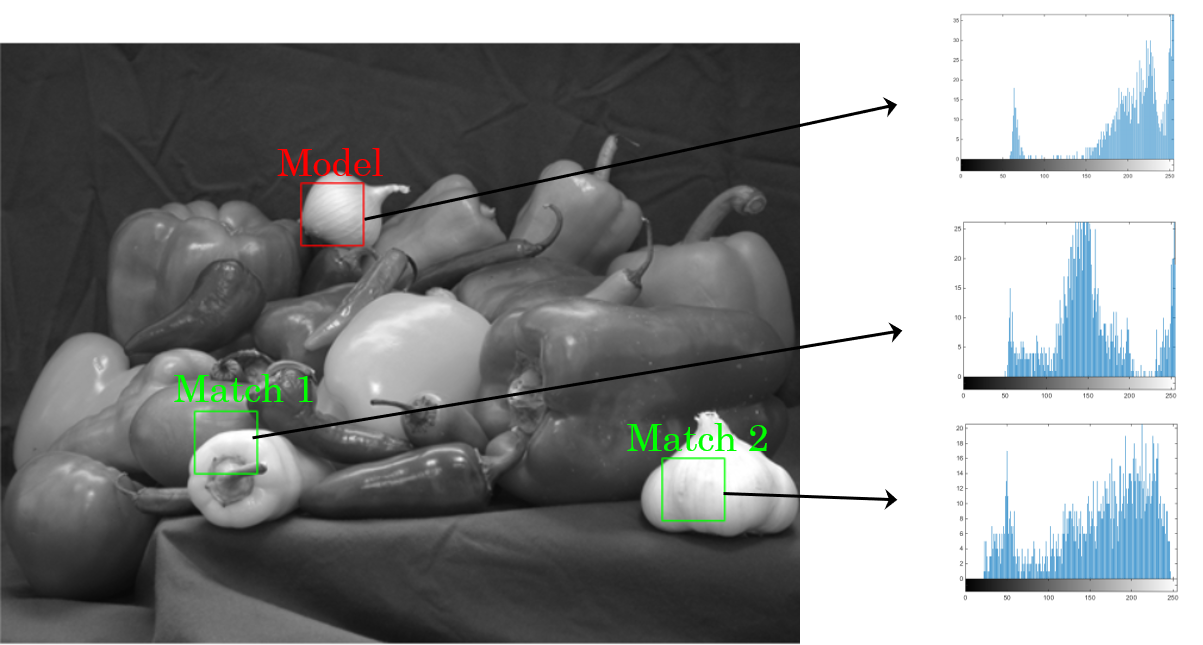
\includegraphics[height=6.5cm]{img/image_hist_different_regions.png}
    \caption{Model and two matches' greyscale histograms.}
    \label{fig:peppers_and_garlic}
\end{figure}


\subsubsection{(optional) The rationale behind defining the ratio histogram}

We assume that 
\begin{enumerate}
    \item the model's histogram (the object we search for) is narrow and tall
    \item and the scene's (whole input image) histogram is rather wide.
\end{enumerate}
It has then been proven (it won't be discussed in this article how as the how is out of scope) that a good histogram similarity measure between the model $M$ and a patch of the image we search it in $I$ is the ratio histogram $R$. $M$ and $I$ need to be pre-calculated and can be divided element-wise, since they have the same range and bins to obtain $R$. The \emphasis{ratio histogram} is a therefore function $R:\mathbb{Z}^2 \rightarrow \mathbb{R}$ that maps a colour $(h,s)$ to some value. If $M(h,s) > I(h,s) \Rightarrow R(h,s) > 1$ that means the model has more pixels of colour $(h,s)$ relative to its total number of pixels compared to $I(h,s)$, and vice versa. If $R(h,s) = 1$, then that means  that the input and model images contain $(h,s)$ at the same degree.

However, because of assumptions (1), (2), $M(h,s) > I(h,s)$ can happen quite often and so long as $M(h,s) > I(h,s) \Rightarrow R(h,s)>1$, e.g. $R(h,s) = 2,3,10$, the exact value does not give much useful information. To summarise, $R$ de-emphasises pixels with colours that do not belong to the model and emphasises the rest.


\subsubsection{A colour matching heuristic}

From the previous section, the conclusion is that it is desirable to clip the ratio histogram to 1, as defined by Swain et al. 
\begin{definition}
For each bin $j$, the ratio histogram is defined as
\begin{equation}
    R_j = \min\left(\frac{M_j}{I_j},1\right)
\end{equation}
, where $M$, $I$ are the model's and input's histograms respectively.
\end{definition}
Note that $j$ does not necessarily have to be a pair $(h,s)$, but it if a histogram bin (index) is quantised it can be a rectangle in the 2D space, such as $[20, 39] \times [50, 69]$. As mentioned before, $R$ associates a colour with its probability of appearing in the model and the next step is the associate each pixel with that probability.

Each pixel of the original image at $(x,y)$ maps to a 2D HS value, by a colour function $c: \mathbb{Z}^2 \leftarrow \mathbb{Z}^2$, by taking $c(x,y)$. Sometimes need an intermediate function $h:\mathbb{Z}^2 \rightarrow \mathbb{Z}^2$ that takes the output of $c$ and quantises it (groups multiple colours in one bin), before it is fed to $R$. For example, $h$ could convert $[0,1,\ldots,179] \times [0,1,\ldots,255]$ to $[0, 19, 39, \ldots,179] \times [0, 24, 49, \ldots, 255]$. The output of $h$ is bed to $R$, which divides $M_j$ to $I_j$ at each bin $j$.To summarise this paragraph we have  defined the following functions in backpropagation:
\begin{itemize}
    \item $c: \mathbb{Z}^2 \rightarrow \mathbb{Z}^2$: maps a pixel at $(x,y)$ to an HS value $(h_j,s_j)$.
    \item $h: \mathbb{Z}^2 \rightarrow \mathbb{Z}^2$ maps a set of values $(h_i,s_i,h_{i+1},s_{i+1},\ldots,h_n,s_n)$ to another $(h,s)$ value by having quantised the range of $h$ and $s$.
    \item $R: \mathbb{Z}^2 \rightarrow [0,1]$ maps an $(h,s)$ value to a probablity.
\end{itemize}
We therefore want to create a new image $b$ where each pixel $(x,y)$ gets assigned its output of $R$ - the measure of how much its colour appears in the model image. 
\begin{equation}
    b(x,y) := R\left(h\left(c(x,y)\right)\right)=
    \min\left(\frac{M\left(h\left(c(x,y)\right)\right)}{I\left(h\left(c(x,y)\right)\right)},1\right) \; \forall \; x,y
\end{equation}
The final step is to find compact regions where $b$ is high. If the shape of the object (model) to detect is generic, then this can be done by convolving $b$ with binary disk mask $D^r$ of radius $r$. Define:
\begin{equation}
    D_{x,y}^r = \left\{
\begin{array}{ll}
      1 & \sqrt{x^2+y^2\leq r} \\
      0 & \textup{otherwise}\\
\end{array} 
\right. 
\end{equation}
Then the probability image $b$ can be convolved with the mask:
\begin{equation}
    b := D^r \ast b
\end{equation}
The $\arg \max$ function to returns the pixel $(x, y)$ with
the maximum value of its argument, i.e. where the $R$ matrix and the $\ast$ symbol denotes convolution. Then Histogram Backprojection can be
written
\begin{algorithm}[H]
\caption{Colour matching by histogram backprojection according to Swain et al}
\label{alg:hist_backproj}
\begin{algorithmic}[1]
\Procedure{Hist-BackProj} {ImM, ImI} \Comment{ImM: model, ImI: search image}
\State $M\leftarrow \textup{histogram}(ImM)$
\State $I\leftarrow \textup{histogram}(ImI)$
\For{each histogram bin $j$} \Comment{a bin is a pair $(h,s)$}
\State $R_j = \min\left(\frac{M_j}{I_j}, 1\right)$ \Comment{Divide element-wise}
\EndFor
\State $m \leftarrow rows(M)$
\State $n \leftarrow cols(M)$
\State $b \leftarrow empty_{m \times n}$
\For{y in 0\ldots m-1}
\For{x in 0\ldots n-1}
\State $b_{x,y} \leftarrow R(h(c(x,y)))$ \Comment{b matrix of colour probability}
\EndFor
\EndFor
\State $D^r\leftarrow$ \textup{binary disk of radius r}
\State $b \leftarrow D^r \ast b$ \Comment{Group (by convolving) high probability pixels together.}
\State $x_{obj},y_{obj} \leftarrow \arg \, \underset{x,y}{\mathop{\max }}\,(b)$
\State \textbf{return}  $x_{obj},y_{obj}$
\EndProcedure
\end{algorithmic}
\end{algorithm}

\subsubsection{Histogram backprojection implementation from scratch}

An implementation of Alg. \ref{alg:hist_backproj} has been written in \ref{app:hist_backproj_src}. However, instead of finding the location of the object by the $\arg \max$ function, it applies Otsu's threshold on the $R$ matrix. This automatically selects a threshold $T$ based on the statistics of the histogram of $R$ for which if $R[x,y] < T$, then the pixel at $(x,y)$ is classified as background, else as foreground. Instructions on how to run the implementation code are in \ref{app:hist_backproj_src} and an output is shown below.
\begin{multicols}{2}
    \begin{figure}[H]
        \centering
        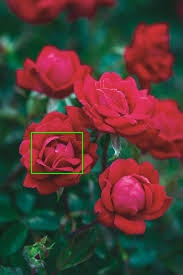
\includegraphics[height=5cm]{img/hist_backproj/rect.jpg}
        \caption{Input image with a ROI of the objects to detect selected.}
        %\label{fig:my_label}
    \end{figure}
    \columnbreak
    \begin{figure}[H]
        \centering
        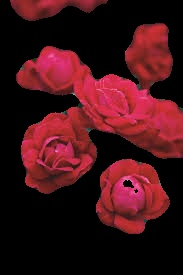
\includegraphics[height=5cm]{img/hist_backproj/res.jpg}
        \caption{Detected objects on the original image.}
        %\label{fig:my_label}
    \end{figure}
\end{multicols}



\subsubsection{Histogram backprojection implementation using OpenCV's API}


OpenCV implements the technique using the \mintinline{python}{cv2.calcBackProject(image, channels, histohram_array, channel_ranges, [scale = 1])} method (in Python). Its invocation looks like:\\
\mintinline{python}{cv2.calcBackProject(search_image, channels, model_histogram, channel_ranges, [scale = 1])}
\begin{itemize}
    \item \mintinline{python}{search_image}: the input image, e.g. in HSV.
    \item \mintinline{python}{channels}: which channels of the original image and the model to select in order to draw its histogram, e.g. \mintinline{python}{channels = [0,1] -> H, S}.
    \item \mintinline{python}{model_histogram}: histogram of the model (ROI), needs to be pre-calculated.
    \item \mintinline{python}{channel_ranges}: set it to \mintinline{python}{[0,180,0,256]} to select the full range of H, S components.
\end{itemize}
The code listing in \ref{app:hist_backproj_src_opencv} works similarly with the one in \ref{app:hist_backproj_src}, expecting two clicks from the user to define a bounding box around a sample of the object to detect. It also performs similarly on the same images, showing some black spots on roughly the same positions.


\subsubsection{Histogram backprojection summary}
\begin{multicols}{2}
    \begin{itemize}
        \item[\textcolor{DarkPink}{\ding{51}}] Fast -- can easily be used in real time.
        \item[\textcolor{DarkPink}{\ding{51}}] Relatively immune to noise and illumination changes.
        \item[\textcolor{DarkPink}{\ding{51}}] Simple to implement.
    \end{itemize}
    
    \columnbreak
    \begin{itemize}
        \item[\textcolor{DarkPink}{\ding{55}}] Not effective against non-compact objects.
        \item[\textcolor{DarkPink}{\ding{55}}] Does not use any knowledge about the shape or position of the detected object -- only its colour.
    \end{itemize}
\end{multicols}





\subsection{Mean Shift Tracking}








%------------------------------ New section ------------------------------%

\section{Motion-based methods}

\subsection{Optical Flow}



\subsection{Lukas-Kanade tracking}



%------------------------------ New section ------------------------------%
\section{Edge-based methods}

\subsection{Hough Transform}






%%%%%%%%%%%%%%%%%%%%%%%%%%%%%%%%%%%%%%%%%%%%%%%%%%%%%%%%%%%%%%%%%%%%%%%%%%%%%%%%%%%%%%%%%%%%%%%%%%%%
% APPENDICES
%%%%%%%%%%%%%%%%%%%%%%%%%%%%%%%%%%%%%%%%%%%%%%%%%%%%%%%%%%%%%%%%%%%%%%%%%%%%%%%%%%%%%%%%%%%%%%%%%%%%
\newpage
\appendix

\section{Appendices}

% ------------------------ New appendix ------------------------ %
\newpage
\subsection{HSV domain}
\label{app:hsv_domain}






% ------------------------ New appendix ------------------------ %
\newpage
\subsection{Histogram implementation from scratch - source code}
\label{app:hist_backproj_src}
\inputminted{python}{src/hist_backproj/backproj.py}



% ------------------------ New appendix ------------------------ %
\newpage
\subsection{Histogram implementation using OpenCV - source code}
\label{app:hist_backproj_src_opencv}
\inputminted{python}{src/hist_backproj/backproj_cv.py}


\end{document}